\subsection{Estimating Bathymetry}

In this Section, we describe some experimental results with simulated and real data using few existing nonlinear optimization tools that we used in our preliminarily experiments (see Section \ref{inv_techniques}). Note that our forward model is nonlinear as described in Section \ref{forwardproblem} and it can not be written as a matrix equation system. Therefore, in this Bathymetry inversion, we can not use any inverting method where it needs forward operator as a explicit matrix operator (e.g., \verb|tikhonov| and  \verb|lsqnonneg|     
 Matlab\textsuperscript{\textregistered} functions need forward operator as a matrix). Moreover, since the bounds of the true Bathymetry is known to be $[0m, 11m]$ 

\subsubsection{Simulated Data}
In this study, Gaussian noise corrupted simulated data (see Section \ref{Gaussian_noise} for more details) is generated by 
\begin{equation}
\mathbf{d}_s = A(\mathbf{h}_t) + \mathcal{N}(0, \nu^2),
\end{equation}
where $A(\cdot)$ represents the nonlinear forward operator defines in Section \ref{forwardproblem}, $\mathbf{h}_t \in \mathbb{R}_+^n$ is the true Bathymetry vector, and $\mathcal{N}(0, \nu^2)$ is a additive Gaussian noise vector with standard deviation $\nu$, generated in the Matlab\textsuperscript{\textregistered} by $\nu \cdot $\verb| randn(n,1)|.
\subsubsection{Real Data}
\begin{figure}[H]
\center
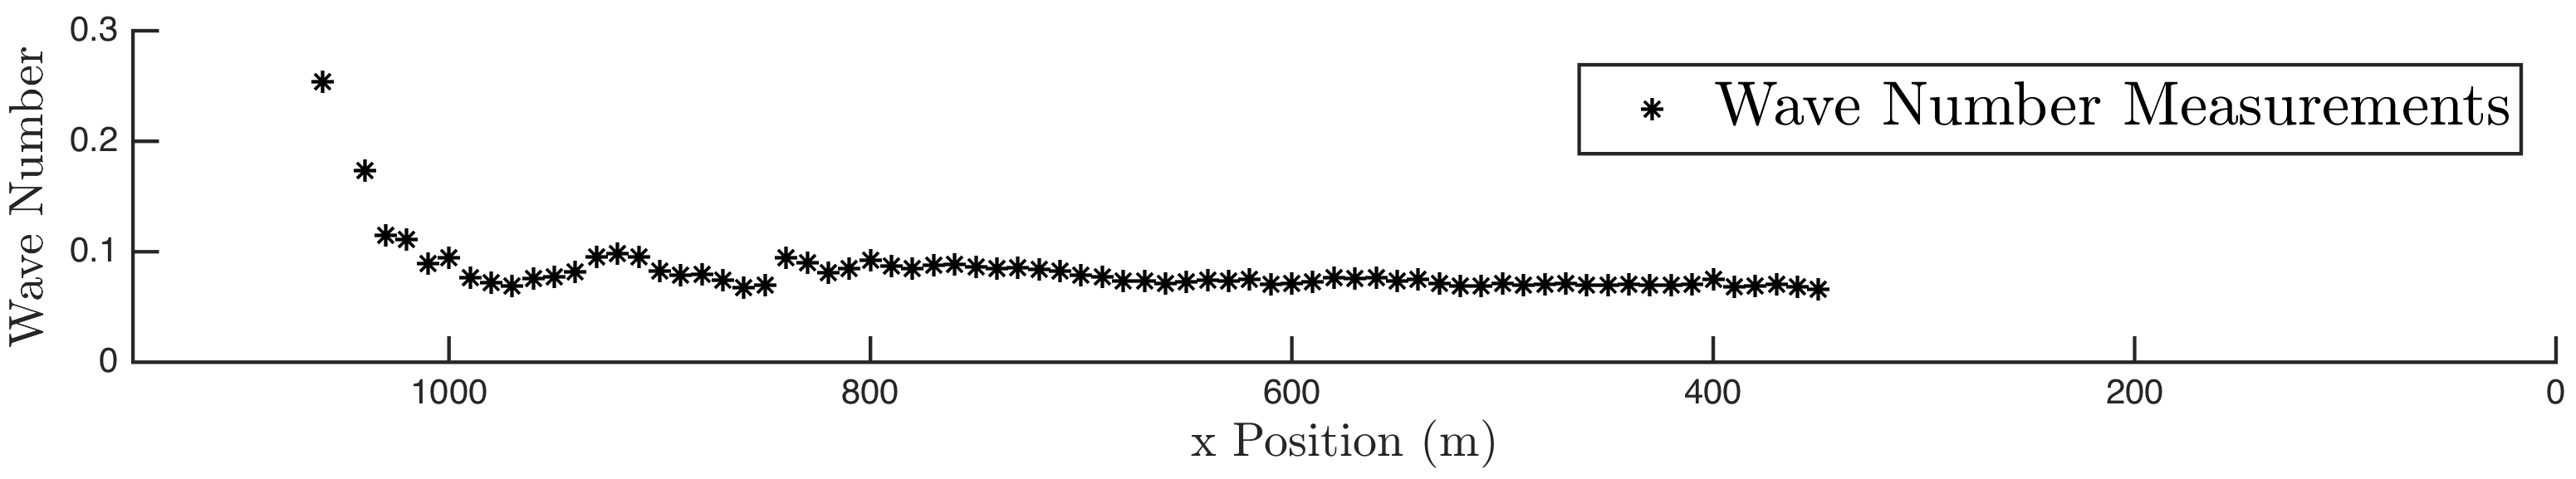
\includegraphics[scale=0.6]{img/real_data_k_Oct09.png} 
\caption{Real data - 09 October 2015}
\label{LM_fig}
\end{figure}




\subsubsection{Ordinary Least-Squares Fitting}

\begin{equation}\label{LS-BC}
\mathbf{\hat{h}}= \underset{\mathbf{0} \preceq \mathbf{h} \preceq \mathbf{11} }{\arg \min} \ \  \|  \mathbf{A}(\mathbf{h}) -  \mathbf{d} \|_2^2,
\end{equation}

[put MCMC results from simulated data and real data sing the Matlab's lsqnonlin function]\\


\subsubsection{Tikhonov Regularization}

\begin{equation}\label{LS-regBC}
\mathbf{\hat{h}} = \underset{\mathbf{0} \preceq \mathbf{h} \preceq \mathbf{11}}{\arg \min} \ \ \|  \mathbf{A}(\mathbf{h}) -  \mathbf{d} \|_2^2  +  \alpha \| \mathbf{h}\|_2^2,
\end{equation}

[Using the Matlab's fmincon function ]


\begin{figure}[H]
\center
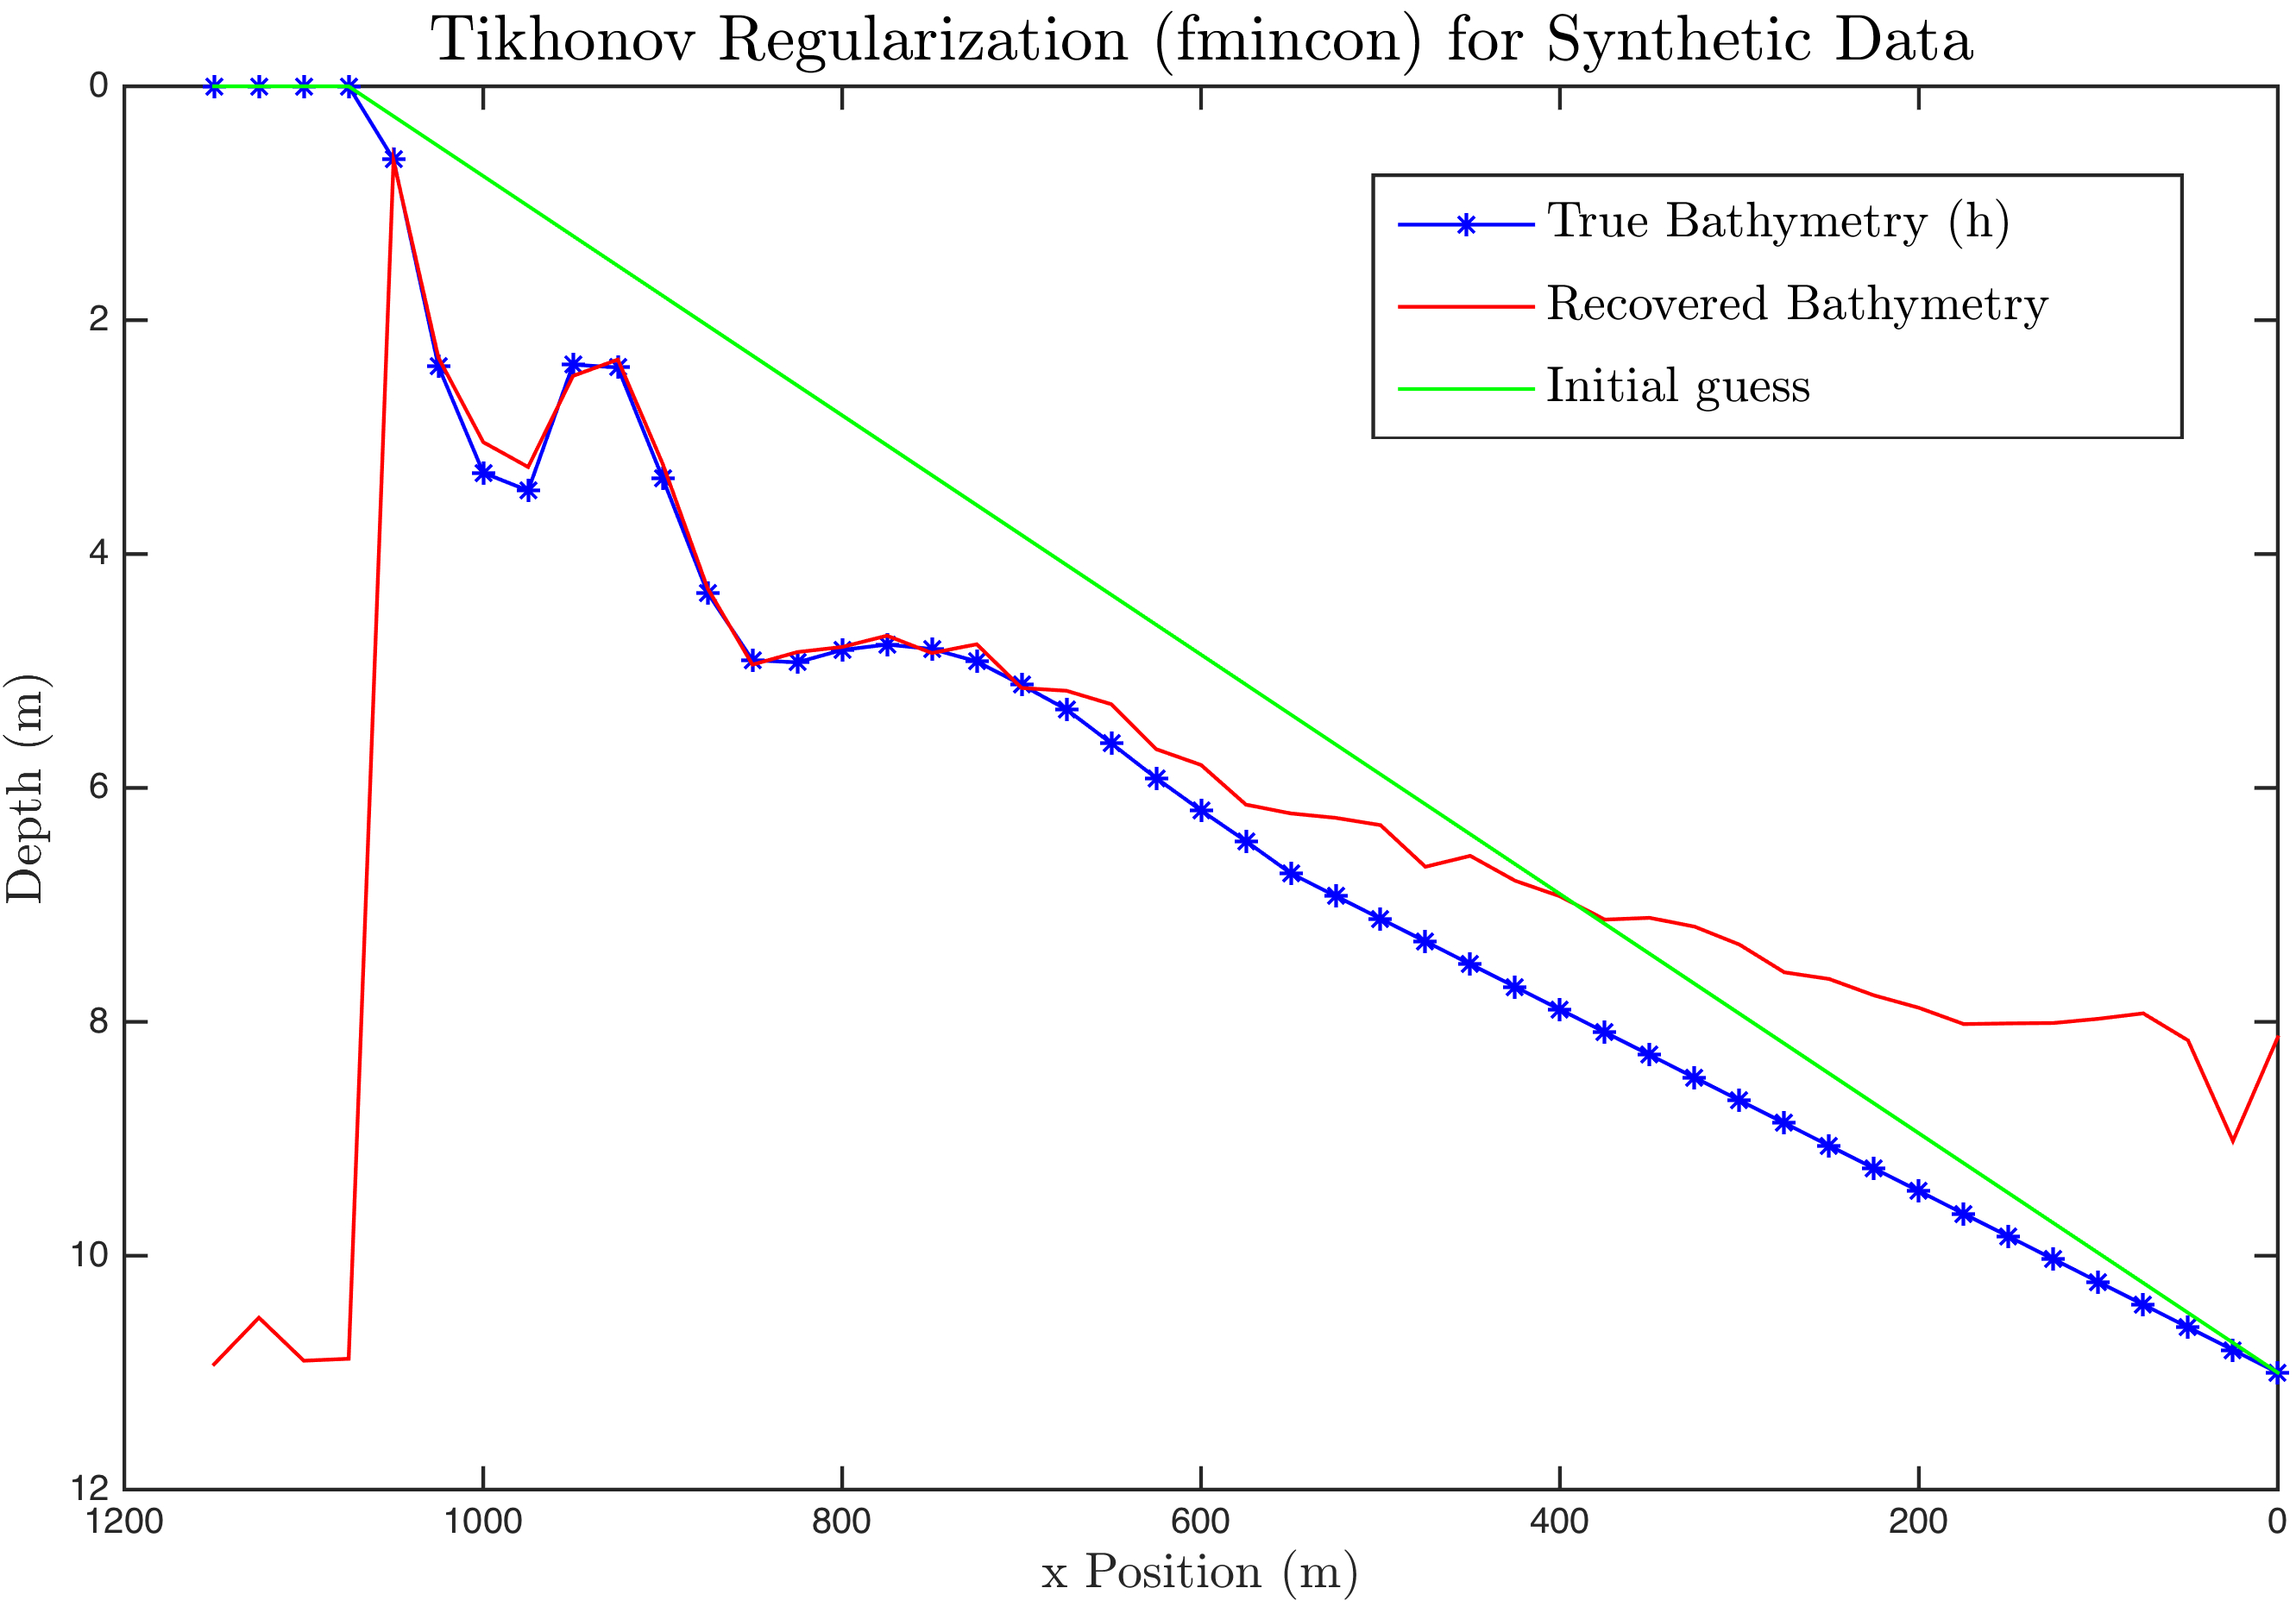
\includegraphics[scale=0.6]{img/fmincon_simulated_25m.png} %plot20 
\caption{fmincon method reconstruction of depth $\mathbf{h}$ using the simulated data.}
\label{fmincon_simulated}
\end{figure}



\subsubsection{Bayesian Inference}
[put MCMC results from simulated data and real data]